\documentclass[a4paper,12pt]{report}

\usepackage[latin2]{inputenc} % vagy latin2 helyett utf8
\usepackage[T1]{fontenc}      % karakterkódolás
\usepackage[english]{babel}   % angol beállítások
\frenchspacing                % helyközök
%\usepackage{times}           % betûtípus
\usepackage{lmodern}          %   vagy inkább ez

\usepackage[margin=2.5cm,left=3.5cm,includeheadfoot]{geometry}
                              % margók
\usepackage{graphicx}         % képekhez
\usepackage{setspace}         % sorköz
\onehalfspacing               % másfeles
\usepackage{hyperref}
\usepackage{listings}
\usepackage{courier}
\usepackage{pdfpages}
\usepackage{amsmath}



\begin{document}

% ------------------------------------------------------------------------------
% Címlap

\begin{titlepage}

\noindent
\parbox[m]{0.2\textwidth}{
%\includegraphics[width=0.2\textwidth]{elte_logo_bw.eps}     % fekete-fehér
 
\includegraphics[width=0.2\textwidth]{elte_logo_color.eps} % színes
}
\hfill
\parbox[m]{0.7\textwidth}{
\begin{center}
\begin{large}
\textsc{
E\"otv\"os Lor\'and University\\
\vspace{0.5pc}
Faculty of Informatics\\
\vspace{0.5pc}
Department of Numerical Analysis\\
}
\end{large}
\end{center}
}

\vspace{1pc}
\hrule

\vfill

\begin{center}
{\LARGE Digital Siganl Processing Plugin\\for Multilayered Synthesis}
\end{center}

\vfill

\noindent
\hspace*{0.05\textwidth}
\parbox{0.45\textwidth}{
{\it Supervisor:}
\bigskip

{\Large Viktoria Zs\"ok}
\smallskip

Assistant Lecturer
}
\hfill
\parbox{0.45\textwidth}{
{\it Author:}
\bigskip

{\Large Evan Sitt}
\smallskip

Computer Science BSc
}


\vfill

\begin{center}
{\large {\it Budapest, 2014}}
\end{center}

\end{titlepage}


% ------------------------------------------------------------------------------
% Témabejelentõ

\vspace*{\fill}
\begin{center}
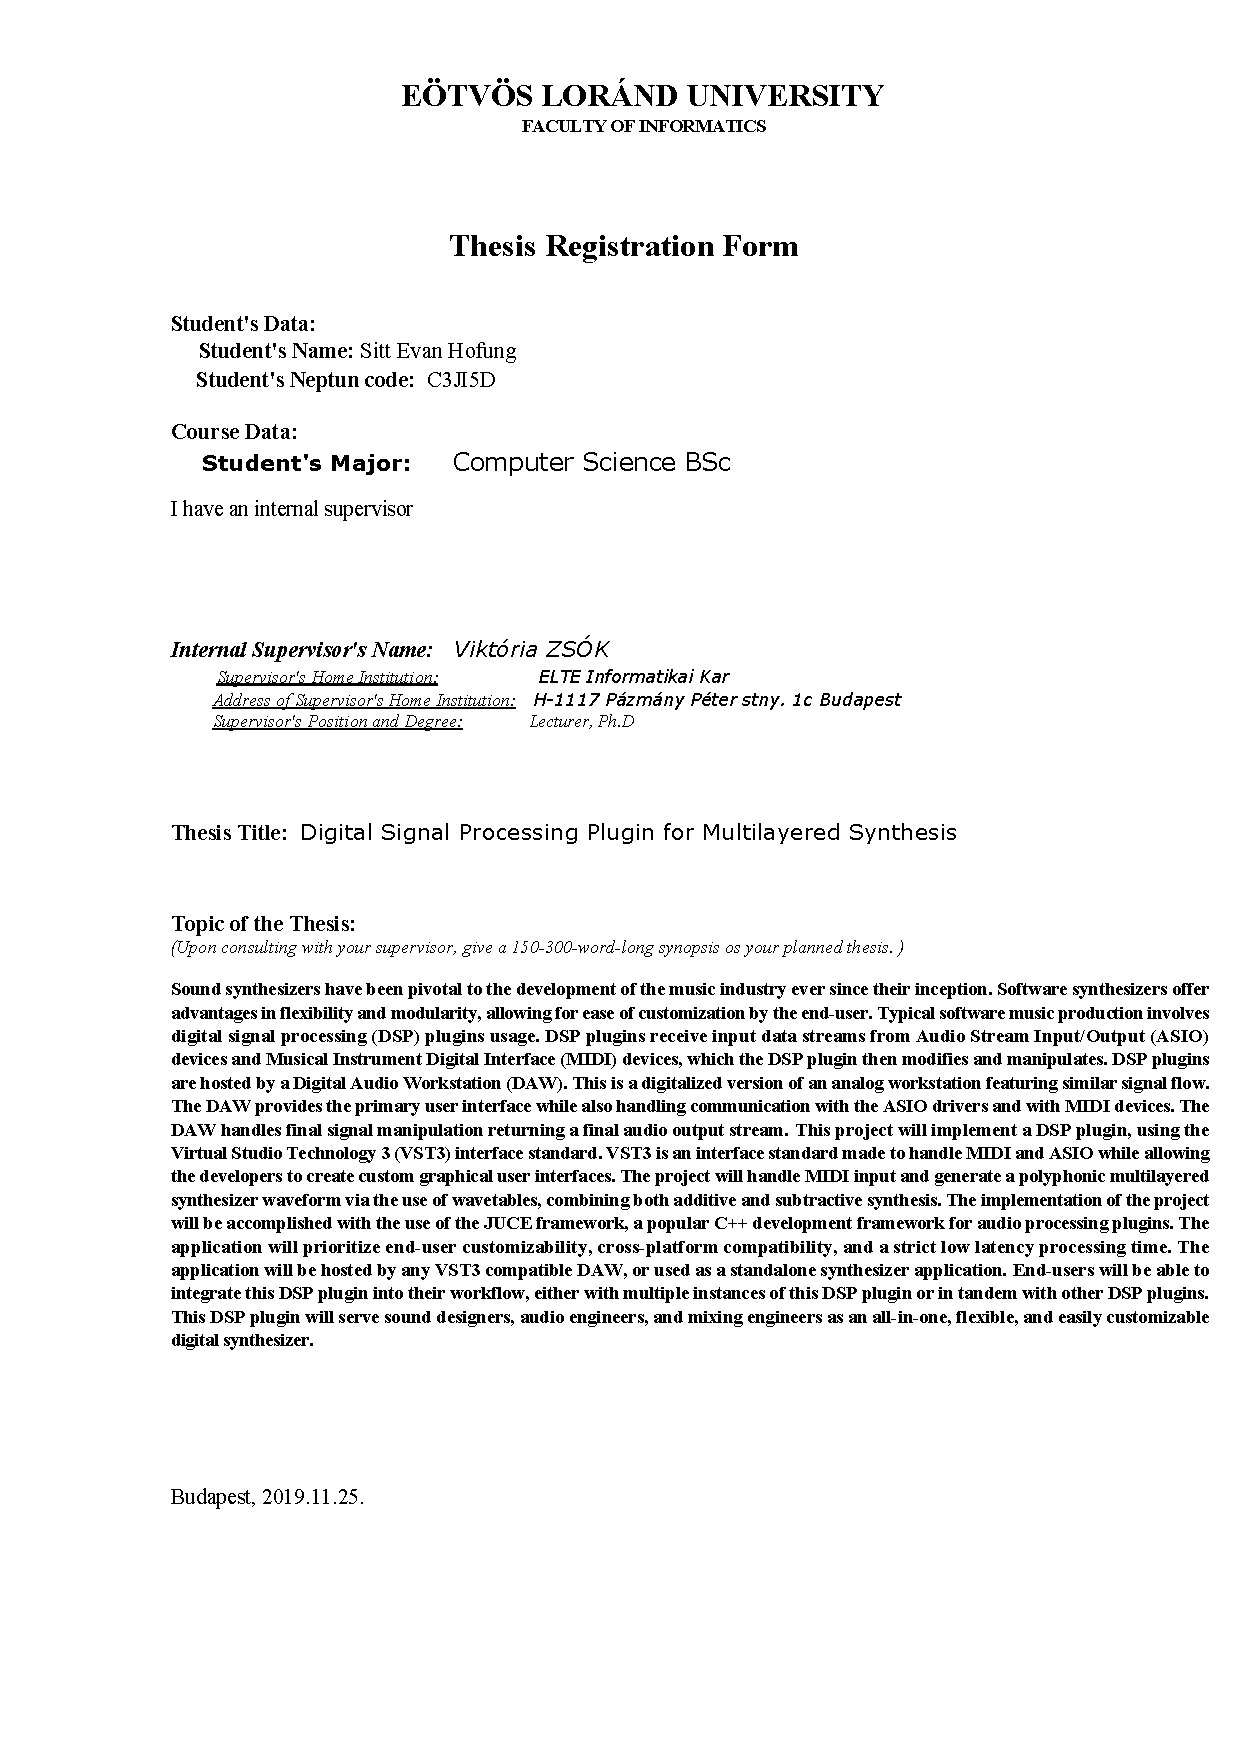
\includepdf[]{Sitt Evan Hofung (C3JI5D); Request identifier-1027058890; Request submission date-11252019 65916 PM}
\end{center}
\vfill
\thispagestyle{empty}
\newpage
\setcounter{page}{1}

% ------------------------------------------------------------------------------
% Tartalomjegyzék

\tableofcontents

% ------------------------------------------------------------------------------


\chapter{Introduction}

The Introduction should summarize the motivation of the topic for the thesis and summary and understandable description of the project.


% ------------------------------------------------------------------------------

\chapter{Background}
\section{Audio Basics}
% - Audio Basics
Before we delve into the background for Digital Synthesis and Digital Signal Processing, it behooves us first to have a brief overview of audio. Audio typically deals with the way we create a sound, the way our ears receives the sound, and the way our mind perceives the sound.

\subsection{Waveform}
We start with the basic building block of sound, the waveform. A Waveform is an abstract way of representing a sound. Typically a waveform is visualized on the Time Domain with Amplitude as the range containing a single cycle of a waveform. Time Domain of a waveform is typically represented in seconds. The Amplitude range, on the other hand, can be represented in many different units. The most common unit used is the decibel (dB). 

\subsection{Decibel}
A decibel is a relative unit of measurement representing the ratio of the value of a power quantity to another. For example, if $x$ represents the ratio of the power quantity of one system to another system, then the decibels can be calculated via $10 log_10 x$. Since the decibel is a relative unit, it is always essential to establish what the reference measure of power is. 

In colloquial usage, when one refers to the loudness of a jet-plane engine as +80dB, this is gin reference to the lower threshold of sound pressure that is perceivable to the human hearing system. In the case that a waveform is referencing the lower threshold of human hearing, then the range is typically visualized with "0" of the range as 0dB and the values above the horizontal axis going up in decibel value and values below the horizontal axis going down in decibel value. A negative value is representative of the vibration of a membrane, such as an eardrum, in reaction to negative sound pressure. 

\subsection{Decibels in Digital Synthesis and Audio Engineering}
In contrast to the colloquial usage of decibels, within audio engineering, the decibel value used is called the Decibels Relative to Overload.  In this variant, 0dB is assigned to the maximal power level that can be output by a system before clipping occurs. Clipping is the term to describe the type of distortion that occurs when a signal overshoots the maximal output. For example, a speaker representing a sound pressure of 0dB will be outputting the signal at its maximum power, and representing the sound pressure at half power would be -6dB. In hardware, safeguards are implemented at certain decibel levels to curb a signal before it clips.

\subsection{Digital Representation of Decibels}
Within a Digital Synthesis system, the power of a signal is represented using \texttt{float} data types. Typically, $1.0$ would represent the maximal power output, $0.0$ would represent the minimum power output, and $-1.0$ would represent the maximal power output with negative sound pressure. Sound pressure levels between maximal and minimal are represented as decimal values between $0.0$ and $1.0$. As with any floating-point value stored within a digital context, the precision of this value is highly dependent on the number of bits used to store the floating-point value. For the \texttt{PCM\ WAV} standard used for the majority of digital audio synthesis done on computer systems, 8-bit, 16-bit, and 32-bit floating-point values are commonly used.

\subsection{Frequency Domain}
The other commonly used representation of sound is the Frequency Domain representation. Here the frequency is the domain, while amplitude remains as the range. In contrast to the Time Domain, there are no time values within the Frequency Domain. As such, the view of the Frequency Domain graph represents the frequency spectrum and amplitude values at an instantaneous point in time.

Frequency refers to the rate at which a sound repeats a single cycle of its periodic function. The frequency is measured in hertz, which represents $cycles/seconds$. Human hearing is capable of perceiving sound with frequencies between 20Hz and 20kHz. While the actual range of any one person's audible range will vary depending on their age, health, and several other factors, the majority of sound reproduction systems will operate within the full range between 20Hz and 20kHz. 

\subsection{Frequency Spectrum}
The graphical representation of the Frequency Domain of a sound is usually referred to as the $Frequency\ Spectrum$ or the $Spectral\ Graph$. These graphical representations will typically represent frequencies between 20Hz and 20kHz, with amplitudes from 0dB to -$\infty$dB. The varying values of the Frequency Spectrum of any waveform control the timbre, or sonic characteristics, of the resulting sound.

A variation on the Frequency Spectrum that is used in digital audio synthesis is the $Harmonics\ Graph$. The Harmonics Graph also represents the Frequency Domain of a waveform. However, the domain represents values from 0 to $\infty$. These do not represent any specific frequencies; instead, the values in the domain represent multipliers of a base frequency. Integer multiplier values are referred to as the $harmonics$ of a sound. A Harmonics Graph represents the unique character of a specific sound-producing object, such as a person's vocals chords, regardless of the frequency of the sound being produced. Harmonics Graphs are commonly used for physical modeling of instruments, which is then later used in reconstructing that sound in Digital Synthesis with the weighted summation of primitive sine waves.


\section{Digital Synthesis}
% - Digital Synthesis
Digital synthesis is a field in which an audio engineer utilizes digital signal processing techniques to make musical sounds. One of the most prominent early examples were the keyboards manufactured by Yamaha, which employed their proprietary FM Synthesis algorithms back in the 1970s.

A frequency synthesizer refers to a synthesizer with circuitry capable of generating a range of frequencies from a single reference frequency input. One typical application of a frequency synthesizer is the use of a Fourier Series to construct waveforms via Additive Synthesis.

\subsection{Direct Digital Synthesis}
% - Direct Digital Synthesis
When designing a digital synthesizer, there is a multitude of techniques available to the designer for generating frequencies, including Phase Locked Loop, Digital-Analog Conversion, and Direct Digital Synthesis. This project approaches the problem of digital synthesis by using Direct Digital Synthesis. Direct Digital Synthesis is a technique utilized by modern frequency synthesizers. Direct Digital Synthesis utilizes a singular fixed-frequency reference clock as a stable time basis for the entire system. In contrast to the alternative Phase-Locked Loop system, where the output phase is locked directly to the phase of the input signal, Direct Digital Synthesis holds significant advantages in flexibility, the most prominent being better frequency agility. Frequency agility is defined as the capacity to switch the oscillator between different frequencies without introducing a significant delay in the signal. This advantage is offered as a result of Direct Digital Synthesis using discrete sample operations. Other advantages offered by the Direct Digital Synthesis technique include access to a broader spectrum of frequencies and finer frequency resolution. Additionally, a Direct Digital Synthesis device has the potential to have low overhead and power draw.

A Direct Digital Synthesis device typically consists of a few parts: a digital signal input, a phase accumulator, a phase register, a phase to amplitude converter, a digital to analog converter, and finally the reference oscillator.

\subsection{Digital Signal Input}
%   - Digital Signal Input
The digital signal input acts as the Tuning Word for the system. The demanded frequency value is provided as an input to the system. Additional information that can be provided at this stage of the system includes the type of waveform to be generated, along with any MIDI instructions for the other signal processing modules further down the signal chain.

\section{Phase Accumulator}
%   - Phase Accumulator
The Phase Accumulator holds the digital number, which represents the current phase of the Direct Digital Synthesizer. The Phase Accumulator iterates the phase with a value controlled by the Tuning Word input. The frequency and sampling rate make up the Tuning Word. Once the phase stored overflows a specified threshold value, modulus mathematics is used to reset the phase within the range specified. With a higher frequency, the Tuning Word will cause the Phase Accumulator to cycle through the phase range more rapidly, in essence accomplishing the task of converting the frequency input into a phase value. In a way, the Phase Accumulator can be thought of as a modulus counter.

%   - Phase Register
\section{Phase to Amplitude Converter}
%   - Phase to Amplitude Converter
After the Phase Accumulator step, the phase value is then passed to the Phase to Amplitude Converter. The goal of the Phase to Amplitude Converter is to change the phase value to a digital amplitude value, which can then be further processed. This goal can be accomplished via two different methods: a Phase/Wavetable lookup, or a Waveform Function.

\subsection{Phase/Wavetable Lookup}
%     - Phase/Wavetable Lookup
The Phase/Wavetable Lookup method was developed in the late 1970s as a more efficient method of generating waveforms on low spec hardware devices. The concept relies on the efficiency advantage of accessing values from a stored array over repeated mathematical calculations of sinusoidal functions. While the hardware constraints are no longer an issue for modern digital synthesizers, the technique is still used for its relative flexibility when compared to the use of sinusoidal functions.

For the Phase/Wavetable Lookup method, a wavetable is stored within the system. This wavetable is named so since it contains a predefined number of precomputed amplitude values of the desired waveform. Typically this waveform is a fundamental sine wave, as other waveforms can be achieved via Fourier series reconstruction, which relies on additive and subtractive operations rather than trigonometric functions. Additionally, the wavetable is typically stored within a direct-access data structure such as arrays for even better efficiency.


For each phase value received from the Phase Accumulator, the Phase to Amplitude converter will use the Phase Register to convert the phase to its respective index value in the wavetable. The amplitude value stored at this index value is retrieved from the wavetable and returned. Since the index value generated typically falls between two integer values, usually some form of numerical interpolation is used. The final amplitude value will then be passed on to the rest of the digital signal processing chain.

The Phase/Wavetable Lookup method holds significant advantages that contribute to its popularity and continued usage. The efficiency of constant time complexity generation of each sample combined with the flexibility to store any waveform allows for nearly unbeatable processing speed for waveforms.

\subsection{Waveform Function}
%     - Waveform function
The other method for Phase to Amplitude Conversion is the use of a Waveform Function. Typically Waveform Functions are used whenever the waveform to be generated can be computed with simple additive and multiplicative computations. Examples of waveforms that typically fit this are the sawtooth and triangle waveform types, as they contain linear sections. Another use case for Waveform Functions is in the case of the square and noise waveform types. In both cases, the resulting amplitude values can be "computed" via without involving any mathematics.

An advantage of using a Waveform Function to convert the Phase to Amplitude is that there is generally no need for interpolation, which results in more accurate amplitude value results. However, as there is typically some form of calculation involved, this method is generally less efficient than the Phase/Wavetable lookup method by a small margin.

\section{Additive \& Subtractive Synthesis}
% - Additive/Subtractive synthesis
After the Phase to Amplitude conversion, the resulting amplitude value is passed down for Additive or Subtractive synthesis. Additive and Subtractive synthesis are exactly what their names imply; they involve the use of additive/subtractive operations between waveforms to create a new waveform. Applied in a systematic method, distinct types of waveforms can be formed.

One method is to use the Fourier series approximation of a waveform. For example, the square wave can be generated via a weighted summation of harmonics of a sine wave. Starting with a fundamental sine wave at a base frequency, we add to this sine waveform each odd harmonic. A harmonic of a waveform is the waveform with a frequency at an integer multiple of the base frequency of the original waveform. The amplitude of each odd harmonic is multiplied by the reciprocal of the harmonic's frequency multiplier in relation to the base frequency.

Another method is to use additive and subtractive synthesis to replicate sounds found in real life, a technique called physical modeling. For example, a piano's sound can be characterized by analyzing a spectral graph of its frequencies. Afterward, this data can be used to generate a set of base frequency multipliers and amplitude multipliers. An Additive/Subtractive synthesizer will then use this set of frequency and amplitude multiplier values to replicate the sound of the piano with high accuracy. This use of Additive and Subtractive synthesis for physical modeling is the technique used and popularized by the Yamaha synthesizers in the 1970s.

\section{LFO}
% - LFO
After the Additive and Subtractive synthesis processes generate a signal for the desired waveform, this is then passed on to the Low-Frequency Oscillator Controlled Modulation processes. Usually referred to as LFO's, these are modulation processes where a value produced by an oscillator modifies the value being modulated. This oscillator typically generates values using a basic sine wave. However, any waveform can be used, resulting in particularly interesting sound characteristics.

Of particular interest are the two most commonly used LFO's: the amplitude LFO and the frequency LFO. Both will modulate their respective parameters using the value from the low-frequency oscillator. An amplitude LFO will reproduce the effect of a tremolo, while the frequency LFO will, on the other hand, reproduce the effect of a vibrato. LFO's can be further controlled by processing the signal from the control oscillators in the same manner as a standard oscillator, although in general, this processing is typically limited to just an Envelope.

\section{Envelope}
% - Envelope
After the LFO processes the signal, it is then sent to the Envelope. An Envelope is a generalized term describing a function or set of values that control the modulation value of a certain characteristic of a digital signal. Envelopes can be applied to many different types of modulation, including amplitude modulation and frequency modulation. An envelope can also be applied to the frequency and amplitude multiplier values used within Additive and Subtractive synthesis for further refined sounds.

\subsection{ADSR}
%   - ADSR
The majority of digital synthesizers employ an Amplitude Modulation Envelope. These types of envelopes focus on modifying the amplitude of the sound over time, producing unique characteristics in sound, which can cause a synthesizer to produce the sound of a guitar vs. a violin. The simplest and most widely used envelope type is the ADSR envelope. ADSR stands for Attack-Decay-Sustain-Release, as these are the four parameters that the Envelope modifies.

The Attack phase starts from the noteOn MIDI instruction and determines the amount of time required for the amplitude of the sound to transition from silence to its full value as determined by the MIDI velocity. After the Attack phase completes, the Decay phase begins, which acts in opposition to the Attack phase by determining the amount of time required for the amplitude to decrease down to its Sustain level. The Sustain level controls what percentage of the maximum amplitude the sound should be allowed to reach for the duration of the note. And finally, upon receiving a noteOff MIDI instruction, the Release phase begins, which determines the amount of time required for the sound amplitude to decrease back to silence.

These four values can drastically shape the character of a synthesizer's sound. For example, let us say we have produced a proper approximation of a string instrument sound via Additive and Subtractive synthesis. Using an Envelope with a long Attack phase, short Decay phase, high Sustain level, and long Release phase could produce a sound akin to a Cello played legato. On the other hand, using an Envelope with an almost instantaneous Attack phase, a minuscule Decay phase, low Sustain level, and a medium-length Release phase could produce a sound closer to that of an Acoustic Guitar. With proper control of the Envelope parameters, it is possible to replicate many different instruments and styles of playing.

Typically, the Envelope is considered the end of the Digital Signal Generation chain. The Digital Signal Generation chain will then accumulate the samples into an Audio Buffer that is sent to the Digital Signal Processing chain after it is filled.

In the Digital Signal Processing Chain, the order of the processes within the chain is entirely flexible and typically customizable by the end-user to best fit the sound they wish to generate. Additionally, the processes can be applied either in series or in parallel, depending upon the architecture of the synthesizer and the underlying framework. Setting up the Digital Signal Processing circuits in parallel holds an advantage for normalizing audio data to avoid artifacts and peaking, the term used for when the power or amplitude audio signal overloads the design capacity of the system. However, setting up the Digital Signal Processing circuits in series can avoid significant phase-shift issues that can occur from the asynchronous nature of parallel processes. The Digital Signal Processing effect types discussed in the following pages are presented in their serial order within the application.

Digital Signal Processing effects can be categorized into three primary archetypes: Frequency-Based, Time-Based, and Amplitude-Based. Digital signal processing effects within each archetype deal primarily with that domain of the digital signal; however, there are frequently overlapping. For example, a simple reverberation effect is a Time-Based effect. However, more sophisticated reverberation effects will incorporate Frequency-Based effects to create a "shimmering" capability for the reverberation. A Multiband Compressor is also a common Amplitude-Based effect that will incorporate Frequency-Based filters to selectively modulate the amplitude from different parts of the frequency spectrum.

\section{Filters}
% - Filters
Multiple types of Frequency Domain filters can be implemented. Each of these filters operates within the Frequency Domain, best visualized with the instantaneous point in the digital audio signal represented within the Frequency vs. Amplitude domains. In the Frequency Domain, modulation takes place to the amplitude of various frequencies along the frequency response spectrum. 

The various Frequency Domain filter types include the Low, High, and Band Passes, the Low and High Shelves, and the Peaking filter. Each of these types has a different characteristic of how they affect the incoming audio signal. These types, in turn, changes the timbre, or characteristic quality, of the sound produced. The details will be discussed in the following parts. However, it is good to note that despite the multitude of variations that exist, these are all additive or subtractive combinations of the basic Pass filters.

Additionally, there are a variety of designs for audio filters. These designs, while initially made for analog systems, work exceptionally well for Digital Signal Processing as well. Each of these designs has differences in their properties that affect the character of the resulting audio signal filter. The most important properties are the Frequency-Domain Ripple factor, the Roll-Off, and finally, the Resonance.

The Frequency-Domain Ripple factor describes the amount of periodic variation in insertion loss with the frequency of a filter, an unavoidable side-effect of certain mathematical functions such as the notable Chebyshev polynomials which commonly used in polynomial interpolation. Some filter designs will utilize mathematical functions that can minimize or completely eliminate the Frequency-Domain Ripple as these ripples in frequencies causes undesirable audio artifacts in the resulting filtered audio signal.

The Roll-Off property of an audio filter design refers to the steepness of the transfer function with frequency, or in other words, the rate at which the amplitude changes with respect to frequency.  Differing audio filter designs will have different capabilities for Roll-Off, with some mathematical functions such as the Elliptic functions being capable of accomplishing much steeper Roll-Off in contrast to other mathematical functions that can only support gentle slow Roll-Off. While a Roll-Off with a steeper value can be desirable for precise audio signal filters, a Roll-Off with a gentler value can be desirable for the more natural-sounding resulting audio signal.

The most common audio filter designs used are the Butterworth filter, the Chebyshev filter, and the Elliptic filter. Each of these audio filter designs has its advantages and trade-offs for each property. For example, the Butterworth filter design, also known as the maximally flat magnitude filter, holds the sole advantage over the other design types in that the Butterworth filter design has no Frequency Domain Ripple in the frequency response graph before the Roll-Off, however, the Butterworth filter design can only support slow and gentle Roll-Off with low Resonance values. By drastic contrast, the Elliptic filter design can support the steepest Roll-Off and the highest Resonance values. However, the Frequency Domain Ripple for Elliptic filters can quickly produce undesirable artifacts.

Typically a synthesizer will be designed around whichever filter design best fits the sound design goal and hardware limitations. More sophisticated and capable synthesizers may utilize complex Audio Filters, which combine multiple filter designs to produce a hybrid design that can mitigate the disadvantages of each design. Within this project, the Butterworth filter design is used exclusively for all Audio Filter types for its ease of implementation, lack of audio artifacts, and efficiency.

\subsection{Low Pass Filter}
%   - Low Pass
A Low Pass Filter is the most commonly used variant of the Pass type filters. A Low Pass Filter will attenuate the amplitude of signals with frequencies higher a set Cutoff frequency to $-\infty$ dB and pass signals with frequencies lower than the Cutoff frequency. The resulting sound will have a "darker" or "smoother" timbre. A Low Pass filter can also be instrumental in helping remove certain high frequencies that can be too harsh for some people.

An everyday use of a Low Pass filter within a music workflow is to apply it to a synthesizer that is being utilized as a bass synth, with the cutoff frequency set to somewhere around 100hz. In this manner, the Low Pass filter will pass through the relevant bass frequencies while filtering out the higher frequencies that may interfere with the desired frequencies of the other instruments.

\subsection{High Pass Filter}
%   - High Pass
The High Pass filter works in exact opposite to how the Low Pass filter operates. While a Low Pass filter will pass frequencies lower than the target cutoff frequency while filtering out those frequencies higher than the target cutoff frequency, the High Pass filter will do the opposite. A High Pass filter can help eliminate common low-frequency rumbles within recordings.

High Pass filters typically are used for vocal recordings where the low-end frequencies caused by vibrations to the microphone or recording setup produce undesirable sounds. Alternatively, a High Pass filter can be used to isolate specific high-frequency instruments, a triangle, for example, so that they can be processed separately.

\subsection{Band Pass Filter}
%   - Band Pass
When a High Pass filter is combined with a Low Pass filter, a Band Pass filter is created. A Band Pass filter will filter out frequencies within a certain range of the "cutoff" frequency while passing all frequencies outside of this range. The Band Pass filter is desirable for its ability to filter out a specific set of frequencies, and with a small enough range, even remove close to one single frequency.

This functionality of the Band Pass filter is commonly used to eliminate noise and clean up synth waveforms. In recordings, it is common that a particular machine will cause noise at a specific frequency throughout the duration of the recording. By determining the frequency of this noise and filtering it with a Band Pass filter, it is possible to remove noise effectively. The Band Pass filter can help with Additive Synthesis as well, as there are many instances when two waveforms will have constructive interference at a specific frequency that may cause distortion. The Band Pass filter will help remove these distortions.

By combining a variety of the three types of pass filters, an Equalizer is created, which can drastically alter the character of a waveform and is a staple of Digital Sound Processing platforms, including consumer-level products.

% - Time-Based Delays
%   - Delay Chain
%   - Flanger

\section{The MIDI Standard}
% - MIDI
MIDI is an acronym for \emph{Musical Instrument Digital Interface}. Originating in 1983 from a panel of music industry representatives, it is a technical standard that describes a universal digital communications protocol for connecting any type of audio-related hardware and software. Analog hardware relies on converters that translate MIDI messages into analog control voltages. 

A single MIDI link is capable of carrying up to sixteen channels of MIDI information. The routing of each channel can be completely independent of each other, allowing for flexible routing to and from different devices. Modern hardware and software will extend this functionality by using ports, with the current standard being 255 ports supported. Each port will support a full set of sixteen MIDI channels, making for a total of 4,080 available MIDI channels useable by the device.

Each MIDI channel is responsible for transmitting MIDI event messages. These event messages typically contain data that specify instructions for music such as a note's notation, pitch, velocity, panning, pitch bend, and tempo. However, in many cases, devices will send and receive proprietary MIDI event messages that can contain instructions for anything, ranging from automating and triggering other devices to controlling performance lights and pyrotechnics. One notable example is the use of MIDI to connect the music playing to a crowd to a fireworks display in a manner that synchronizes well and is automated.

\subsection{MIDI Event Messages}
\includegraphics[width=1.0]{MIDIInstructionsTable.needed}

MIDI event messages consist of 8-bit byte-words transmitted in series at a rate of 31.25 kilobits per second, a rate chosen for being an exact divisor of 1 MHz. Each byte-word starts with a bit indicating if the word is a status byte or a data byte. The next seven bits encode the relevant information or instruction. On top of the 8 bits forming the byte-word, a start bit and a stop bit are used to frame the byte-word, summing up to a total of ten bits per byte-word in transmission.

Each MIDI event message contains an instruction for which the receiving device may choose to act upon. The two main categories of MIDI event messages are Channel event messages and System event messages. A device can choose to act upon or ignore any or all MIDI event messages received.

Channel event messages contain instructions that usually are relevant to the audio to be produced. A \texttt{noteOn} message will indicate to the device that a note has started. Similarly, the \texttt{noteOff} message indicates that the note has ended. On a keyboard, these two MIDI event messages would correspond to the pressing of a key and the release of the key. Channel event messages can also convey pitch information in the form of MIDI notation. MIDI notation assigns the integers from 0 to 127 to all possible notes within the music. This range of integers corresponds to the range from $C1$ up to $G9$ according to the Helmholtz pitch notation standard, covering a range of frequencies from 8.175798916 Hz to 12,543.85395 Hz. This range of possible notes and frequencies extends well beyond the range of the majority of acoustic instruments. Another important piece of information that Channel event messages can convey is the \texttt{velocity} value of a note. The \texttt{velocity} value corresponds to how forcefully a note was played, corresponding to the $piano$ and $forte$ notation instructions on traditional sheet music. The \texttt{velocity} value typically will control the loudness of the sound generated, but may also control other parameters such as resonance and vibrato. For digital synths, the \texttt{velocity} value of a note can be used to control different modulations. The Channel event messages can also contain tempo and time signature instructions. These correspond to their musical notation equivalents and combine with the beat value of a note to determine the time value of the note. The beat value is conveyed in the Channel event messages via the \texttt{duration} value. Each \texttt{duration} unit within MIDI notation corresponds to $1/24^{th}$ of a beat value. There is also a large variety of other Channel event messages; however, the essential Channel event message types have been discussed.

System event messages are used to promote the flexibility and longevity of the MIDI communication standard by allowing manufacturers to create proprietary event messages. These System event messages allow for devices to communicate instructions typically corresponding to other software or hardware control parameters. For hardware and analog systems, a converter will translate the MIDI System event message to control voltage values. There are no universal standards for System event messages. However, with modern MIDI software and hardware systems, there are commonly used standards established by widely used software.

\subsection{MIDI Channels and Ports}
Each MIDI link between devices is capable of carrying up to sixteen channels of MIDI information. The MIDI channels are identified with a binary encoding with values from $0$ to $15$. However, to the End-User, these are presented as the numbers 1 to 16. MIDI ports extend a device's MIDI link capacity. These MIDI ports are identified with hexadecimal encoding with values from $0$ to $255$. MIDI-compatible hardware and software support 16 MIDI channels of information, but they may choose to listen or ignore any number of these MIDI channels. On the other hand, the implementation of MIDI ports is dependent upon the constraints of the software or hardware and is more commonly found on modern devices.

The application of this thesis project supports one MIDI link of sixteen channels, with all MIDI channels being handled at the same time. System event messages are ignored, as the application is not device or platform-specific, nor does it use proprietary interfaces. However, most MIDI event messages are handled by the application.

%   - Handling the buffer
\section{Waveform Audio File Format}
% - PCM Wav
%   - Handling the buffer

\section{Digital Audio Workstations}
% - Digital Audio Workstations

% 7 - 10 pages Background
% May 1st Deadline, 45 days left.
% ------------------------------------------------------------------------------

\chapter{User Documentation}
In this chapter, the application will be explained from an End-User perspective with explanations on how to use each part of the application within their workflow to achieve the desired sound. This section will rely heavily on technical and musical terminology discussed in the previous chapter \ref{ref:needed}, and as so, will focus primarily on describing in detail the operation and effects of the application.
% The User Documentation (or User's Manual) should contain
% \begin{itemize}
% \item the short description of the solved problem,
% \item the summary of the used methods and tools,
% \item every required information about the usage of the software.
% \end{itemize}

\section{Installation}
The installation of the software is relatively straightforward and simple. This section will walk the End-User through the Build, Installation, and Setup process on different platforms. For those who prefer to download the precompiled binaries for the VSTi plugin, please read the following subsection. However, for those who prefer to build the application from the source code, please refer to section \ref{ref:needed}.

\subsection{Installing the VSTi}
The latest release builds of the VST3 plugin can be found at \href{link:needed}{text:needed}. Once downloaded, the installation of the plugin within the preferred Digital Audio Workstation will proceed as specified by the specific Digital Audio Workstation. Typically, the process consists of placing a copy of the VST3 plugin binary within the designated system folder for VST3 plugins and registering the new plugin within the Digital Audio Workstation. The Digital Audio Workstation must support ASIO drivers, MIDI input, and VSTi 3.0 plugins.

For the purposes of demonstration, the $FL\ Studio\ 20$ Digital Audio Workstation running on the $Windows\ 10$ operating system will be shown and referenced in the instructions.

\includegraphics[width=1.0]{FLStudioLogo.needed}

\subsection{Registering the VST3 Plugin}
The first step to installing the VST3 plugin is to copy the \texttt{.vst3} file into the appropriate directory set in the $Plugin\ Manager > Plugin\ search\ paths$ field. By default, the directory set for 64-bit plugins on 64 bit Windows 10 is typically found in the \texttt{'../Program Files/Common Files/VST3'} directory. 

Afterward, the user should open the $Plugin\ Manager$ via the $Options$ by going to $File\ settings$ and then clicking on the $Manage\ plugins$ button. 

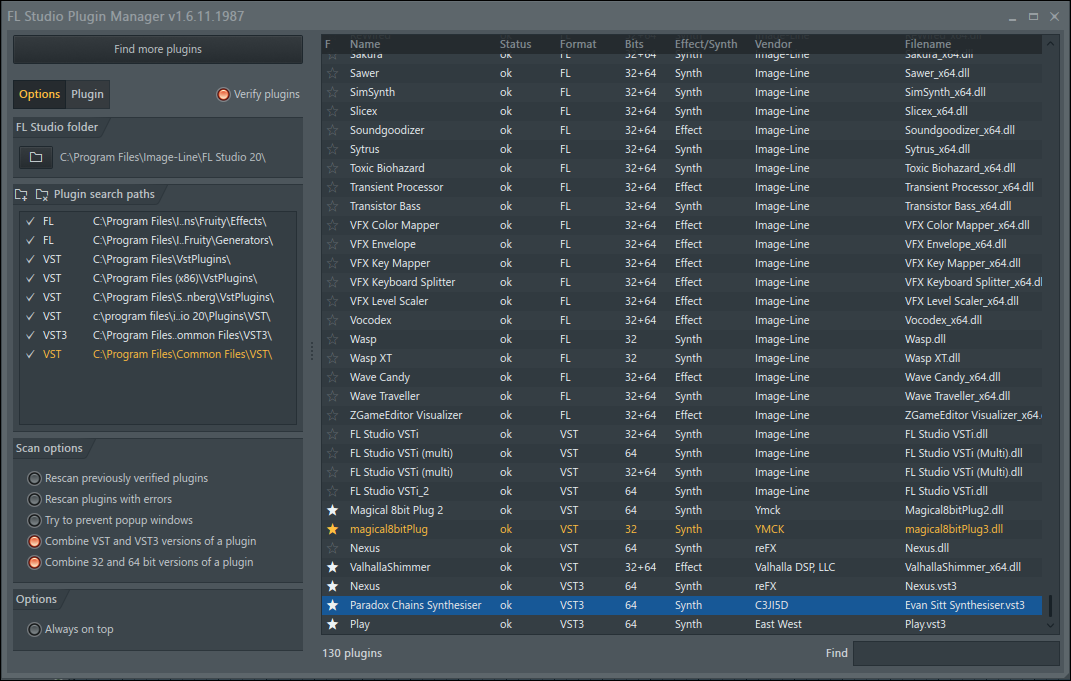
\includegraphics[width=1.0]{ModuleRegistration.needed}

After ensuring that the $Verify\ plugins$ radio button is turned on, the next step is to use the $Find\ Plugins$ button to scan the preregistered VST plugin folders for the new VST3 plugin. The window will then show the new plugin, named $Paradox\ Chains\ Synthesiser$, within the plugin list on the right panel. By selecting the star button next to the plugin name, the plugin will be added to the favorites to ensure ease of finding the plugin in the future. This last step completes the registration of the VST3 plugin within the FL Studio 20 Digital Audio Workstation.

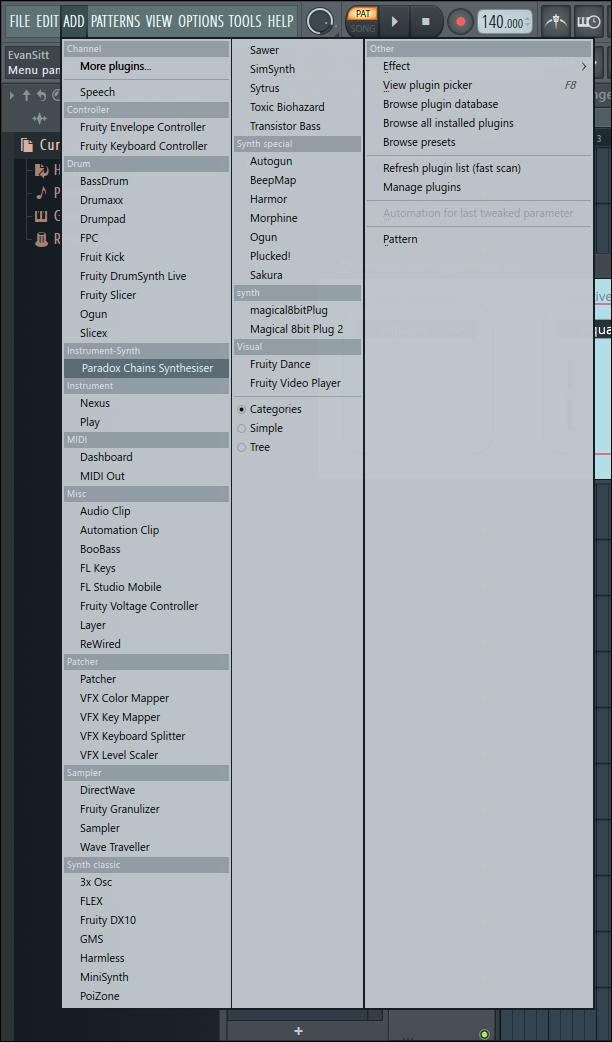
\includegraphics[width=1.0]{AddPluginList.needed}

\section{Initialization and Workflow Integration}
While the previous steps stated in the $Installation$ section \ref{Reference.needed} will only need to be completed once, the steps in this section and the following $Workflow\ Integration$ section \ref{reference.needed} will be the steps necessary to be taken for every new project established.

To add an instance of the VST3 plugin to a project, simply go to the $Add$ dropdown menu in the top left, and then select the $Paradox\ Chains\ Synthesiser$ option. This action will automatically add an instance of the VST3 plugin to the $Channel\ rack$. The $Channel\ rack$ can be accessed via $'View\ >\ Channel\ rack'$ or via the $F6$ shortcut key. By clicking on the VST3 plugin within the $Channel\ rack$, the user can access the graphical user interface of the synthesizer.

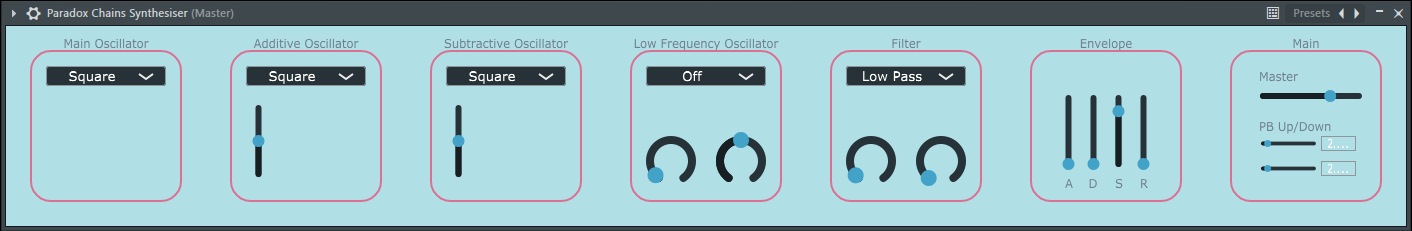
\includegraphics[width=1.0]{SynthesiserMainGUI.needed}

Each outlined portion of the graphical user interface of the VST3 plugin contains the controls which correspond to a process within the Digital Signal Processing chain. The specifics of each module will be discussed in the $Module\ Details$ section /ref{ref.needed}. Controls on the main user interface can be set during a project or modified in real-time during a performance as the situation demands. The Digital Synthesis Processes will automatically read in the new parameters and adjust the sound accordingly.

The full list of detailed controls, with labels and fine controls, can be accessed by advanced users via the $Browser$ panel on the left side of the screen. By using the center $Current\ project$ tab, opening up the $Generators$ listing, and then opening up the $Paradox\ Chains\ Synthesiser$ listing, the advanced user will have access to all possible MIDI values for the VST3 plugin.

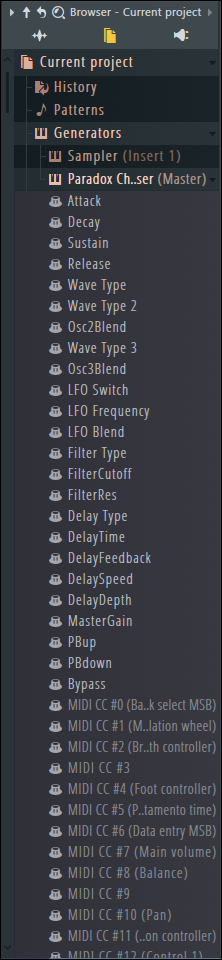
\includegraphics[width=1.0]{BrowserPanel.needed}

Clicking on any one of them will bring up a detailed rotary slider that will also display a precise value to pass to the VST3 plugin. Note, the value displayed by the Digital Audio Workstation is from a range between $0.0$ and $100.0$, corresponding to the percentage of the range of the MIDI parameter. However, as detailed within the $Module\ Details$ section \ref{ref.needed}, the actual value range of the MIDI parameters will be different depending upon the parameter.

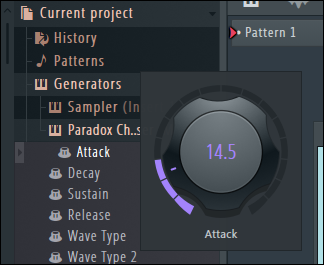
\includegraphics[width=1.0]{ModifyingDetailedMIDI.needed}

Right-clicking on any of the detailed MIDI parameters will bring up advanced user options. The $"Init\ song\ with\ this\ position"$ option will allow the advanced user to set the current value as an initialization value. The $"Edit\ events"$ option will allow the advanced user to enter a detailed MIDI event graphical editor window. The $"Create\ automation\ clip"$ option will allow the advanced user to create tracks to automate the MIDI parameter. Lastly, but certainly not least, the $"Link\ to\ controller"$ option will allow the advanced user to link the MIDI parameter, or even the entire VST3 plugin, to either a software control panel, such as FL Studio's $Patcher$, or even a hardware MIDI device.

\includegraphics[width=1.0]{ExtraOptions.needed}

The final step to integrating the $Paradox\ Chains\ Synthesiser$ into a workflow is to route the digital audio output to the mixer. By opening up the VST3 plugin's graphical user interface, there is an option to click on the Settings button to bring up the detailed settings window. There is a multitude of options, such as modifying the MIDI input and output ports; however, the relevant option is to change the Track Assignment in the top right corner of the window. By changing this value, the VST3 plugin will be assigned to the corresponding mixer track for further processing and routing to the final output.

\section{Module Details}


\begin{itemize}
    \item Installation
    \item Initialization
    \item Workflow Integration
    \item Module Details
    \item Testing details
\end{itemize}

% ------------------------------------------------------------------------------


\chapter{Developer Documentation}

% The Developer Documentation (or Developer's Manual) should contain
% \begin{itemize}
% \item the detailed specification of the problem,
% \item the detailed description of the used methods, the definitions of the used notions,
% \item the description of the logical and physical structure of the software (data structures, databases, modules, etc.),
% \item the testing plan and the results of the tests.
% \end{itemize}

\section{Prerequisites}
Before developing the code, the developer must have access to a few necessary tools.
\begin{itemize}
\item The Project Source Code, available from Github.
\item The JUCE C++ Application Framework
\item A development environment of your choice. JUCE natively supports Visual Studio, XCode, and Linux Make.
\item A Digital Audio Workstation of your choice. It must support VST3 plugins.
\end{itemize}
\subsection{Building the Software from Source Code}
The stable source code of this application can be downloaded from the \texttt{master} branch of the public repository found at Github: \href{https://github.com/ParadoxChains/C3JI5D-Evan-Sitt-BSc-Thesis}{https://github.com/ParadoxChains/C3JI5D-Evan-Sitt-BSc-Thesis}. The source code includes all of the $C++$ header and CPP files that are necessary for the application. However, the repository does not include the JUCE framework that is required for building the project.

\subsection{JUCE Framework}
The JUCE framework is a partially open-source, cross-platform C++ application framework. It is particularly notable for its robust support of the VST3 SDK providing developers with an easy toolset for interacting with VST3 applications. Additionally, the JUCE framework provides graphical user interface functionality, supports a large variety of integrated development environments and compilers, and is designed to compile and run compatibly on the Windows, Mac OS X, and Linux platforms.

The JUCE framework is required for the project as it provides the base framework for interacting with the VST3 SDK. The JUCE framework can be found on the Roli JUCE website at: \href{https://juce.com/}{https://juce.com/}. The project for this application will work with both paid, free, and GPL licenses for JUCE. The Projucer application, a necessary extension of the JUCE framework, can be downloaded along with the framework. Further details on setting up the JUCE framework and Projucer application can be found on the JUCE website.

% maybe more details on JUCE setup?

\subsection{VST3 Standard}
The JUCE framework's main strength is the robust support for working with the VST3 SDK. This acronym stands for the Virtual Studio Technology audio plugin interface developed by Steinberg Media Technologies. 


\includegraphics[width=1.0]{VST3Logo.needed}

VST Plugins are designed to work in conjunction with a Digital Audio Workstation, or with a similar standalone wrapper application providing the same functionality. VST Plugins are generally categorized into two categories: Generators and Effects. A subcategory of the Effects category exists for the sole purpose of visualization and data representation called Visualizers. VST Plugins typically have an integrated graphical user interface for ease of use, presenting the End-User with controls that mimic their physical equivalents on audio hardware. However, many VST plugins have controls for advanced users that do not have a graphical user interface and rely on the host application or Digital Audio Workstation for the user interface.

The Generator category of VST plugins typically consists of digital synthesizers. These are software simulation emulations of audio synthesizer hardware, typically incorporating similar signal flows and processes, however, usually, optimizations are made in consideration to the nature of digital synthesis. 

The Effects category of VST plugins differs from the Generator category in that they do not generate new audio signals. Instead, they modify an existing audio signal. As such, these VST plugins typically do not take MIDI input or produce MIDI output, but only deal with audio signal input and output. Similar to the Generator category of VST plugins, Effect VST plugins are software simulation emulations of their respective audio synthesizer hardware equivalents.

Many modern VST3 plugins are a hybrid of the Generator and Effect types. These VST3 plugins will typically receive MIDI input, generate new audio signals from the MIDI instructions. Afterward, the VST3 plugin would process those audio signals in tandem with signals received from the audio input before passing the finalized audio signal to the audio output. The application developed for this thesis falls within the Generator/Effects hybrid category of VST plugins and provides a simplified graphical user interface for the entry-level user while making the advanced controls accessible from the Digital Audio Workstation.

The VST standard specifies a standard for communication between Digital Audio Workstations and the VST Plugins. The standard includes communication of MIDI input and output, audio signal input and output, and parameter value input and output. The VST Plugin will specify to the Digital Audio Workstation which inputs are available. Based upon the inputs received from the Digital Audio Workstation, the VST Plugin will process this information and then send various output messages back to the Digital Audio Workstation. These output messages can go directly to the Digital Audio Workstation or can be directly passed on to other VST Plugins, creating a signal chain. As such, \emph{chaining} is a useful technique for connecting VSTs to form deeply layered and sophisticated sounds.

\section{Process Flow}
The central object which handles the flow of data is the \texttt{AudioProcessor} found within the \texttt{PluginProcessor} header and CPP files. The \texttt{AudioProcessor} is responsible for directing MIDI input and Audio output throughout the different objects. Additionally, the \texttt{AudioProcessor} is responsible for handling the MIDI buffer and Audio buffers. The \texttt{AudioProcessor} will contain instances of the other classes and assists them in interacting with each other.

The front-end of the \texttt{AudioProcessor} that will be used by the End-User is handled by the \texttt{AudioProcessorEditor}. This \texttt{AudioProcessorEditor} object contains each of the individual graphical user interface objects and controls the overall appearance of the VST3 plugin. These individual graphical user interface objects are \texttt{processor} objects that each will contain the individual graphical user interface elements to assist the End-User in changing the state values of the VST3 plugin, such as sliders and rotary dials.

The \texttt{AudioProcessor} also contains an array of \texttt{SynthesiserVoice}. Each of these objects is a Synthesiser object that will perform the computation of values that will be handed back to the \texttt{AudioProcessor}  for sending out to the audio buffer. The \texttt{AudioProcessor} is responsible for handling the MIDI buffer and sending those sets of instructions to the Synthesiser objects for processing.

\section{Development Flow}
While development can follow the flow of the process, it is not intuitive to develop in this manner. To develop the \texttt{AudioProcessor} first would require a complete understanding of which control and state values would be required for each synthesizer component.

First, the developer must develop the functions for handling the MIDI buffer first and the corresponding synthesizer functions. The audio buffer functions must also be developed afterward to handle the output correctly.

Then at this point, the synthesizer components can be created. After this, developing the \texttt{AudioProcessor} to manage the control and state values is much more straightforward. From here, it is advised to develop the graphical user interface for the new synthesizer component, which will connect to the \texttt{AudioProcessor}, and then finally adding it to the \texttt{AudioProcessorEditor}.

Special care must be taken to ensure that all functions are thread-safe, as the JUCE framework makes full use of VST3's multithreading support for performance, especially when handling high polyphony counts.

The following section will walk through the development flow as described and provide detailed instructions on each portion.

\section{Initializing the Synthesiser}
The first step is to set up the \texttt{Synthesiser} controlled by the \texttt{AudioProcessor}. It is sufficient to declare the \texttt{Synthesiser} within the private members and allow it to use its default constructor. 
Within the constructor of the \texttt{AudioProcessor}, we then create a loop that will add new instances of the \texttt{SynthesiserVoice} class and new instances of the \texttt{SynthesiserSound} class to the \texttt{Synthesiser}. The following is the code snippet that performs this action.
\begin{lstlisting}
mySynth.clearVoices();
    
for (int i = 0; i < 5; i++)
{
    mySynth.addVoice(new SynthVoice());
}
mySynth.clearSounds();
mySynth.addSound(new SynthSound());
\end{lstlisting}
The \texttt{clearVoices} and \texttt{clearSounds} methods ensure that we are starting with a fresh \texttt{Synthesiser}.

\section{Handling the MIDI and Audio Buffers}
There are two parts to the handling of MIDI input and audio output. The \texttt{AudioProcessor} must implement a \texttt{processBlock} function. This function is called by the framework at every tick of the program, and is passed the references to the \texttt{AudioSampleBuffer} and the \texttt{MidiBuffer}. The following is the declaration required for this function:
\begin{lstlisting}
void JuceSynthFrameworkAudioProcessor::processBlock (AudioSampleBuffer& buffer, MidiBuffer& midiMessages)
\end{lstlisting}
Within the \texttt{processBlock} function, the developer may choose to implement any sort of system-wide functionality that must occur in real-time. One of these functionalities is the retrieval of control and state values from the \texttt{AudioProcessorValueTreeState}, which will be discussed in detail in a later section \ref{ref.needed}.

The first step is to ensure that a call is made to the \texttt{renderNextBlock} method of each \texttt{SynthesiserVoice} that was added to the \texttt{Synthesiser}. These calls are done within a loop that iterates through each \texttt{SynthesiserVoice}. The function call is as follows: 
\begin{lstlisting}
mySynth.renderNextBlock(buffer, midiMessages, 0, buffer.getNumSamples());
\end{lstlisting}
Within the \texttt{renderNextBlock} function call, the audio buffer and MIDI buffer are both passed in by reference, followed by the index of the starting sample and the index of the last sample.

Within the \texttt{SynthesiserVoice} derived class we must implement an override on the \texttt{renderNextBlock} method. The function declaration is as follows:
\begin{lstlisting}
void renderNextBlock(AudioBuffer <float>& outputBuffer, int startSample, int numSamples) override
\end{lstlisting}
This method must accomplish the task of rendering and adding the audio output sample values to the provided \texttt{AudioBuffer}. The code within this consists of two nested loops, one which iterates through each sample of the \texttt{AudioBuffer}, and the other which iterates through each audio channel that needs a sample. Within the loops we call an \texttt{AudioBuffer} method, \texttt{addSample}, to add the new sample to the \texttt{AudioBuffer}. The code snippet is as follows:
\begin{lstlisting}
for (int sample = 0; sample < numSamples; ++sample)
{
    for (int channel = 0; channel < outputBuffer.getNumChannels(); ++channel)
    {
        outputBuffer.addSample(channel, startSample, giveSample());
    }
    ++startSample;
}
\end{lstlisting}
The first argument is the channel index, the second argument is the sample index, and the last argument is the value to be written. To keep the code readable and maintainable, the value to be written is provided by the function \texttt{giveSample}. This function will be described in further detail in the subsection \ref{ref.needed}.

\section{The Digital Synthesis Components}
The next parts for the developer to build are the individual Digital Synthesis components. The usage and purpose of each component have been discussed in the $Module Details$ section \ref{ref.needed}, and this section will focus on the implementation and technical details.

\subsection{Waveform Oscillators}
Designing an oscillator consists of two primary parts: designing the $Phase Accumulator$ as described in \ref{ref.needed} and designing the $Phase-to-Amplitude Converter$ as described in \ref{ref.needed}.

The $Phase Accumulator$ is accomplished by declaring a \texttt{phase} variable for the \texttt{oscillator} class. This value will be used by each of the $Phase-to-Amplitude Converter$ functions. Since each $Phase-to-Amplitude Converter$ function uses the same \texttt{phase} value, it is ensured that the transition between different waveforms can be done with no phasing issues and with relative smoothness.

The \texttt{resetPhase} methods allow for the \texttt{oscillator} to reset the phase to $0$ or to set it to a specified value. The \texttt{iteratePhase} method is responsible for iterating the value of \texttt{phase} by the formula: \begin{math}
\cfrac{\texttt{waveTableSize}}{(\cfrac{\texttt{sampleRate}}{\texttt{frequency}})}
\end{math}

The \texttt{waveTableSize} and \texttt{sampleRate} are constants set by the constructor of the \texttt{oscillator}. The \texttt{waveTableSize} represents the how many precalculated values are stored for a single waveform cycle within a Waveform Lookup Table as described in section \ref{ref.needed}. The \texttt{sampleRate} represents the number of samples to be rendered per second for the audio output. The \texttt{frequency} is a value that will be provided to the oscillator when it is called by the \texttt{SynthesiserVoice} class. By iterating the \texttt{phase} value by the calculated value from the \texttt{waveTableSize}, \texttt{sampleRate}, \texttt{frequency}, the \texttt{phase} can not only accurately represent the phase but also represent the wavetable lookup index.

With the $Phase Accumulator$ completed, the next step is to create the $Phase-to-Amplitude Converter$. In this project, both $Waveform Lookup Tables$ and $Waveform Functions$ are used. Each of the $Phase-to-Amplitude Converter$ functions follow the same conventions in regards to input and output. Each of the functions takes \texttt{frequency} as an argument, which acts as the $Tuning Word$, and returns a \texttt{double} representing the resulting amplitude from the conversion. These will be explained in the following paragraphs.

The \texttt{sine} function operates using a $Waveform Lookup Table$ in order to bypass incurring the repeated computation cost of sine calculations. A precalculated wavetable, \texttt{double sineWaveTable[ ]} is stored within the CPP file. This array contains a predetermined number of precalculated values representing values of one cycle of the primitive sine function with an amplitude of $1$. The size of the wavetable is 4800 values. This number, $4800$, is calculated by dividing the highest possible sampling rate for $PCM WAV$ encoding, $98,000Hz$, by the lowest audible frequency, $20Hz$. While a lower number of precalculated values may be sufficient, some systems use a wavetable with as few precalculated values like 128, having a higher wavetable size ensures for much higher accuracy with less reliance on interpolative accuracy. Additionally, the extra overhead incurred by the memory allocated for a larger array of \texttt{double} values is negligible by the standard of modern computing hardware and is typically not a limiting factor.

The \texttt{sine} function first checks the \texttt{phase} value to ensure that it is within the bounds of the wavetable size. If the \texttt{phase} value is not within these bounds, then modulus mathematics is applied to the \texttt{phase} value to shift it to a value within those bounds. This \texttt{phase} value, as calculated by the \texttt{iteratePhase} method, serves as the access index of the wavetable. As this access index typically will not fall on an integer value, but rather some real number index, the value can not be simply accessed from the wavetable. Instead, the $floor$ of the \texttt{phase} value is calculated and four values are accessed. These values are the value at the floored index, the value immediately following that position, and the two values immediately preceding that position. With these four values, a $4-Point Polynomial Interpolation$ algorithm is used to calculate the final value. The following is the code for the $4-Point Polynomial Interpolation$ algorithm.
\begin{lstlisting}
decimalPlaces = phase - floor(phase);
a = sineWaveTable[(long)phase - 1];
b = sineWaveTable[(long)phase];
c = sineWaveTable[(long)phase + 1];
d = sineWaveTable[(long)phase + 2];
x = 0.5f * (c - a);
y = a - 2.5f * b + 2.0f * c - 0.5f * d;
z = 0.5f * (d - a) + 1.5f * (b - c);
outputValue = double(((z * decimalPlaces + y) * decimalPlaces + x) * decimalPlaces + b);
\end{lstlisting}
The final \texttt{outputValue} is then returned from the function, which will be used for further Digital Signal Processing.

Since the calculation of values for the Saw, Square, and Triangle waveforms involve only elementary addition, subtraction, multiplication, and division, the cost of repeated calculations is far cheaper than repeated sine calculations. For this reason, the $Phase-to-Amplitude Converter$ functions for these waveforms are implemented as $Waveform Functions$.

The \texttt{square} function contains a conditional block which will set the \texttt{outputValue} to either $-1.0$ or $1.0$ depending on the current \texttt{phase} value. It will also perform modulus mathematics to ensure that the \texttt{phase} value is within the value range. Below is the core code block of the \texttt{square} function:
\begin{lstlisting}
if (phase < 0.5 * waveTableSize)
    outputValue = -1.0;
else if (phase >= 0.5 * waveTableSize)
    outputValue = 1.0;
if (phase >= waveTableSize)
    phase -= waveTableSize;
\end{lstlisting}


\subsection{AudioProcessorValueTreeState}
One of the first crucial steps is to build the \texttt{AudioProcessorValueTreeState}, a JUCE framework tree object designed to facilitate the storage of state values of the VST3 plugin and the access and communication of this information between the Digital Audio Workstation and the VST3 plugin.

The \texttt{AudioProcessorValueTreeState} is declared within the header file, and is initialized in the constructor list of the \texttt{AudioProcessor}. The following code block is an example of initializing the filter parameters:

\begin{lstlisting}
tree(*this, nullptr, "PARAMETERS",
        {   
            //Filter Parameters
            std::make_unique<AudioParameterChoice>("filterType",
                                             TRANS("Filter Type"),
                                       StringArray("Low Pass","High Pass","Band Pass"),
                                                  0),
            std::make_unique<AudioParameterFloat>("filterCutoff", "FilterCutoff", NormalisableRange<float>(20.0f, 10000.0f), 400.0f),
            std::make_unique<AudioParameterFloat>("filterRes", "FilterRes", NormalisableRange<float>(1.0f, 5.0f), 1.0f),
        })
\end{lstlisting}

This block will initialize the specified MIDI control value and state values that the VST3 plugin will need to make accessible to the Digital Audio Workstation. Any state value that will only be used and modified internally does not need to be added to the \texttt{AudioProcessorValueTreeState} object.

In each initialization call, a call is made to a \texttt{std::make\_unique<>()} object constructor. This template class constructor will be given a JUCE framework type corresponding to the VST3 standard type. For example, a frequency range for the Low Pass Filter is of type \texttt{AudioParameterFloat}, while a dropdown menu selection for selecting between filter types is of type \texttt{AudioParameterChoice}. The JUCE framework later converts these types to their respective VST3 SDK equivalents.

The \texttt{AudioProcessorTreeValueState} is connected the other classes in order to provide access to the VST3 plugin state. Most notably, the \texttt{processor} objects which contain the graphical user interface elements are initialized with references to state values stored within the tree object.
\begin{itemize}
    \item Short Background of Task
    \item Implementation of Task
    \item Discussion of implementation
    \item Results - Latency, Under/Overruns, Distortion/Clipping
\end{itemize}


% ------------------------------------------------------------------------------

\chapter{Appendix}

% ------------------------------------------------------------------------------

\begin{thebibliography}{9}
\bibitem{v} Somebody, something.
\end{thebibliography}

\end{document}
